\newpage 
\section{Lecture 3: Numerical Analysis of finite difference} 
Recap: 
\begin{itemize}
    \item Heat equation on $\RR$, $u(x,t) = \frac{1}{\sqrt{4\pi t} }\int_{-\infty}^{\infty} e^{-\frac{(x-\xi)^2}{4t} }g(\xi) \, d\xi $.  
    \item Finite difference notation. 
\end{itemize}
Today's topic: 
\begin{itemize}
    \item Truncation error, consistency, stability 
    \item Convergence statement of Lax-Richtmyer equivalence theorem 
\end{itemize}

\vspace{1em}
\hrule 
\vspace{1em}

Our scheme for $u_t = u_{ xx } $ is $D_t^{+} u_j^n=D_x^{+} D_x^{-} u_j^n$. Then we can solve $u_j^{n+1}$ by: 
\begin{align*}
    \frac{1}{h}\left[u_j^{n+1}-u_j^n\right]=\frac{1}{h^2}\left[u_{j+1}^n-2 u_j^n+u_{j-1}^n\right] \Rightarrow u_j^{n+1}=u_j^n+\frac{k}{h^2}\left[u_{j+1}^n-2 u_j^n+u_{j-1}^n\right]. 
\end{align*}
If we let $ \nu = \frac{k}{n^2} $, we have 
\[
    u_j^{n+1}= \nu  u_{j+1}^n+(1-2 \nu ) u_j^n+ \nu  u_{j-1}^n. 
\]


\subsection{Truncation error, consistency and stability}
%────────────────────────────────────────
\begin{definition}
[Scheme and truncation error]
\label{def: Scheme and truncation error}
Scheme is the recipe for advancing the solution from $t_n$ to $t_{n+1}$. Truncation error is defined as what's left over when you plug the exact solution into the scheme. 
\end{definition}
%────────────────────────────────────────
For our scheme, the truncation error is $ \tau_j^n$ s.t. 
\[
    \underbrace{D_{t}^{+} u\left(x_j, t_n\right)}_A=\underbrace{D_x^{+} D_x^{-} u\left(x_j, t_n\right)}_B+\tau_j^n
\]


%────────────────────────────────────────
\begin{note}
In 228A, we include a factor of $k$ in $\tau_n$. Let $ y' = f(y) $, for the Euler method we have: 
\begin{align*}
    \begin{aligned}
        & y\left(t_n+k\right)=y\left(t_n\right)+k f\left(y\left(t_n\right)\right)+\tau_n^{22 8 A} \\
        & \frac{y\left(t_n+k\right)-y\left(t_n\right)}{k}=f\left(y\left(t_n\right)\right)+\tau_n^{228 B}
        \end{aligned}
\end{align*} 
\end{note}
%────────────────────────────────────────
Note that we have 
\[
    \begin{aligned}
        & A=\frac{u\left(x_j, t_n+k\right)-u\left(x_j, t_n\right)}{k}  \\
        & =\frac{\mu+k u_t+\frac{k^2}{2} u_{tt}+\frac{1}{6} k^3 u_{ttt}\left(x_i, t_n+\theta_1 k\right)-u}{k} \\
        & =u_t+\frac{k}{2} u_{tt}+\frac{1}{6} k^2 u_{ttt}\left(x_j, x_n+\theta_1 k\right) \text { (exact formula) } \\
        &
        \end{aligned}
\]
and 
\[
    \begin{aligned}
        & B=\frac{1}{h^2}\left[u\left(x_j+h, t_n\right)-2 u\left(x_j, t_n\right)+u\left(x_j-h, t_n\right)\right] \\
        & =\frac{1}{h^2}\left[   u+h u_x+\frac{h^2}{2} u_{x x}+\frac{h^3}{6} u_{x x x}+\cdots 
        -2 u +u - h u_x+\frac{h^2}{2} u_{x x}-\frac{h^3}{6} u_{x x x}+\cdots \right] \\
        & =u_{x x}+\frac{h^2}{12} u_{x x x x}+\frac{h^4}{720} \left[         \partial_x^6 u\left(x_j+\theta_2 h, t_n\right) 
        +\partial_x^6 u\left(x_j-\theta_3 h, t_n\right) \right]  \\
        \end{aligned}
\]
Hence, we have 
\[
    \tau_j^n=A-B=\left(u_t-u_{x x}\right)+\frac{1}{2}\left(k u_{t t}-\frac{h^2}{6} u_{x x x x}\right)+O\left(k^2+h^4\right)
\]
Since $u(x,t)$ is the exact solution, we have $ u_t = u_{ xx }  $  and $u_{tt} = (u_t)_t = (u_{ xx } )_t = (u_t)_{ xx } =u_{xxxx}$. Hence, 
\[
    \tau_j^n=\frac{h^2}{2}\left( \nu -\frac{1}{6}\right) u_{xxxx} +O\left(h^2+h^4\right), v=\frac{k}{h^2}. 
\]
Specifically, if $ \nu =\frac{1}{6}$, 
\[
    \left|\tau_j^n\right| \leqslant M\left(\frac{k^2}{6}+\frac{h^4}{360}\right)=\frac{M h^4}{135},
\]
where $M = \max_{x,t} |u_{ttt} (x,t)| = \max_{x,t} |u_{xxxxxx}(x,t)|$. Note that here the max is over the stencil. If we want a bound on all the $\tau_j^n$, we take the max over $x\in \RR$ and $0\le t\le T$. One can show that $M\le \max_x |\partial_x^6 g(x)|$, where $ g$ is the initial condition. If $\nu\neq \frac{1}{6}$, we could have stopped sooner in Taylor's theorem with remainder.  We can show 
\[
    \tau_j^n=A-B=\left(u_{t}-u_{x x}\right)+O\left(k+h^2\right) 
\]
and 
\[
    \left|\tau_j^n\right| \leq M\left(\frac{k}{2}+\frac{h^2}{12}\right)=\frac{M}{2}\left( \nu +\frac{1}{6}\right) h^2
\]
where $ M=\max _{|(x, t) \in \operatorname{stencil}}\left|u_{t+}\right|=\max _{\operatorname{stencil}}\left|u_{x x x x}\right| \leq \max _{x \in \mathbb{R}}\left|\partial_x^4 g(x)\right| $.  


\subsection{Lax-Richtmyer equivalence theorem}
%────────────────────────────────────────
\begin{definition}
[Consistent]
\label{def: Consistent}
A scheme is consistent if $\tau_j^n\to 0$ as $k,h\to 0$. We can also specify the rate like first order in time, second order in space, $\tau_j^n = O(k+h^2)$. 
\end{definition}
%────────────────────────────────────────


%────────────────────────────────────────
\begin{note}
A scheme is \textbf{consistent} if the exact solution of the PDE is an approximate solution of the scheme.  A scheme is \textbf{convergent} if the exact solution of the scheme is an approximate solution of the PDE. 
\end{note}
%────────────────────────────────────────


%────────────────────────────────────────
\begin{theorem}
[Lax-Richtmyer equivalence]
\label{thm: Lax-Richtmyer equation}
A consistent finite difference scheme for a well-posed initial value problem is convergent if it's stable. 
\end{theorem}
%────────────────────────────────────────
The setting of Lax-Richtmyer paper is: 
\[
    \begin{cases}
            & u_t=A u \quad(0 \leqslant t \leqslant T) \\
            & u(0)=g
    \end{cases}
\]
which is a linear, constant coefficient ODE in a Banach space $\cB$.  In our case $A = \frac{\partial^2}{\partial x^2}$ and $\cB = BC(\RR)$, the bounded continuous functions. The norm is the max norm: 
\[
    \|g\| = \|g\|_\infty = \sup_{-\infty<x<\infty} |g(x)|. 
\] 
Note that other Banach spaces also work nicely for the heat equation. $L^1(\RR), L^2(\RR)$. 

%────────────────────────────────────────
\begin{figure}[H]
    \centering
    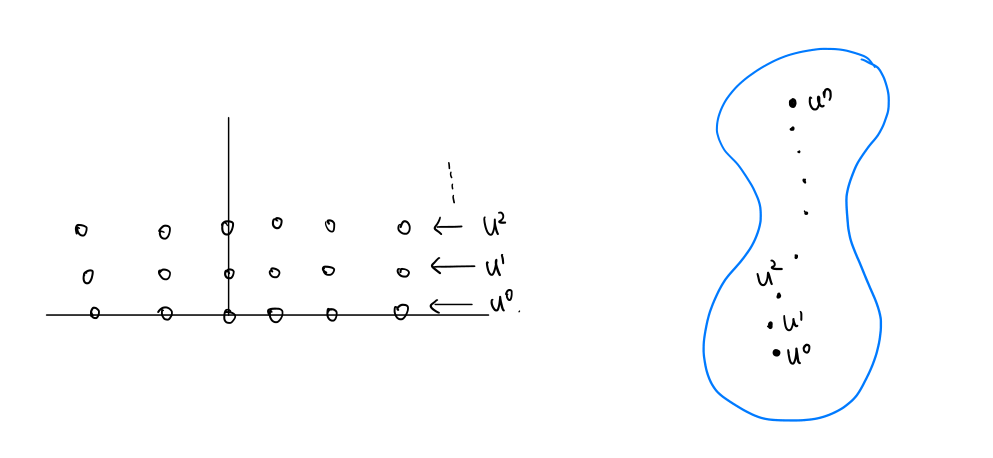
\includegraphics[width=0.8\textwidth]{figures/3-grid.png}
\end{figure}
%────────────────────────────────────────
We can set up a grid and define our finite difference scheme as an operator from one discrete time slice to the next one.  $ \cB_h = l^\infty (\ZZ) = \text{ space of bounded sequences }  \{f_j\}_{j=-\infty}^\infty $. Here we have 
\[
    u^{n+1}=B(k, h) u^n, 
\] 
where $B(k,h)$ is a bounded operator on $\cB_h$.  In our case, 
\[
    B(k, h) u= \nu  u_{j+1}+(1-2 \nu ) u_j+ \nu  u_{j-1}, \quad \nu=\frac{h}{h^2}. 
\]
Next we define a refinement path $h=H(k)$ relating $k$ to $h$. In our case $H(k) = \sqrt{\frac{k}{ \nu }} $.  

Let $B= B(k)$ to denote $B(k, H(k))$.  


%────────────────────────────────────────
\begin{definition}
[Stable]
\label{def: Stable}
A scheme is stable if $\forall T>0, \exists K, \epsilon >0$, s.t. 
\[
    \|B(k)^n \| \le K,
\]
for $0<k<\epsilon $ and $0\le nk \le T$. 
\end{definition}
%────────────────────────────────────────
In our case, $\nu\le \frac{1}{2}$ and $K=1, \epsilon =1$ work for all $T$.  Next time we will prove $\nu >\frac{1}{2}$ then our scheme is unstable.  

